% This is samplepaper.tex, a sample chapter demonstrating the
% LLNCS macro package for Springer Computer Science proceedings;
% Version 2.20 of 2017/10/04
%
\documentclass[runningheads]{llncs}
%
\usepackage{graphicx}
\usepackage{hyperref}
% Used for displaying a sample figure. If possible, figure files should
% be included in EPS format.
%
% If you use the hyperref package, please uncomment the following line
% to display URLs in blue roman font according to Springer's eBook style:
\renewcommand\UrlFont{\color{blue}\rmfamily}

\begin{document}
%
\title{e-Voting on Stellar Blockchain}
%
%\titlerunning{Abbreviated paper title}
% If the paper title is too long for the running head, you can set
% an abbreviated paper title here
%
\author{Stanisław Barański
\inst{1}, Julian Szymanski\inst{1}, Andrzej Sobecki\inst{1}, \\
Higinio Mora\inst{2}, David Gil\inst{2}}

% First names are abbreviated in the running head.
% If there are more than two authors, 'et al.' is used.
%
\institute{Faculty of Electronics, Telecommunications and Informatics\\
Gdansk University of Technology\\
Gdansk, Poland\\
\and
Department of Computer Science Technology and Computation,\\ University of Alicante,  Spain\\
\email{\{stanislaw.baranski%s160518 postaramy sie o email uniwersytecki
,julian.szymanski,andrzej.sobecki\}@eti.pg.edu.gda.pl}
\email{\{hmora,dgil\}@dtic.ua.es}
}

 
\authorrunning{S. Barański et al.}

\maketitle              % typeset the header of the contribution
%
\begin{abstract}
In this paper, we propose an privacy preserving e-voting system based on decentralized Stellar Blockchain network. 
We argue that proposed system satisfy all requirements stated for robust e-voting system such as: transparency, verifiability, and voter anonymity/privacy. 
The architecture of the system 
completely abstracts the voter from used blockchain technology. %  underneath.
To keep the user privacy we propose a privacy-first protocol
that protects  voter anonymity using blind-signature technique, while signer is protected by cut-and-choose method. Open Stellar blockchain allows everyone to verify the election results without having to trust central authority. 
We evaluate our approach 
indicate  the weakness, strengths and possible improvements to achieve an even more robust system. 
 


%JS wypunktować co jest wkładem artykułu
% np slepy podpis

%SB Wydaje mi się że właśnie to:

% production-ready: jest to rozwiązanie, które ma sens wdrażania już dziś. Inne publikacje opierają się albo na bitcoinie (który nie jest przystosowany do tworzenia na nim aplikacji tego typu), albo na Ethereum, który jest o wiele droższy i słabiej się skaluje w dodatku (z tego, co się orientuje), nie da się zaimplementować algorytmu ślepego podpisu w smart contractcie bez ujawniania klucza prywatnego, więc platformy smart contractowe nic tu raczej nie wnoszą. Co więcej, niektóre publikacje zakładają, że każdy głosujący posiada portfel bitcoinowy, co moim zdaniem jest mrzonką. Ten system nie wymaga od użytkownika żadnej wiedzy o blockchainie.

% algorytm ślepych podpisów wydaje mi się, że jest obowiązkowy, chyba każdy artykuł, który chciał zachować prywatność używał ślepych podpisów (były takie które tego nie robiły), nawet w książce Schneiera jest rozdział o systemie do głosowania opartego ślepe podpisy. Więc to nie jest raczej żadna kontrybucja. Co może natomiast nią być to sama implementacja ślepych podpisów, dla schematu EdDSA, którego nie znalazłem zaimplementowanego nigdzie w internecie, a wydaje mi się, że zrobiłem spory research na ten temat. Ostatecznie udało mi się to zaimplementować z pomocą jednego z developerów Stellara, na bazie wpisu na blogu profesora zajmującego się kryptografią (który okazało się, że miał błąd). Nie wiem czy jest to coś co można uznać za naukowy contribution. Na pewno rzemieślniczy contribution, bo poświęciłem na zaimplementowanie tego algorytmu co najmniej 30h :D

% - privacy-first - cały protokół jest stworzony z myślą o prywatności użytkownika. Cokolwiek by się nie działo, prywatność użytkownika jest zachowana. (no, chyba że algorytm ślepych podpisów jest dziurawy)



 
\keywords{Blockchain \and E-Voting \and Stellar \and Tokenization  \and Blind signature}  
\end{abstract}


\section{Introduction}
E-voting has been a topic of research for years, especially in cryptography, which is an inevitable part of the system security. Is seems surprising that in most countries, we still rely on the analog election process, especially in today's level of technology, especially after the Bitcoin convinced that money (which seems to face similar problems) can be done without a central authority. 

%%JS systemy evotingu moga pozwolic wdrozyc koncept demokracji atenskiej w ktorej wszyscy %a nie tylko przedstawiciele maja glos w podejmowaniu decyzji. dyskusyjne czy to dobry pomysl na system polityczny.

% SB rozumiem że chodziło Panu głównie o demokrację bezpośrednią.  Moim zdaniem jest to świetny pomysł, ponieważ zmniejsza to skłonność (jak najbardziej zrozumiałą) do deklaracji obietnic przez polityków. Rola polityków sprowadza się głównie do prowadzenie dyskusji, debat, reprezentacji, zarządzania krajem. Obywatel sam podejmuje decyzję które argumenty przemawiają do niego i na tej podstawie podejmuje głos. Dodatkowo system jest o wiele bardziej elastyczny, wyborca może zgadzać się w niektórych kwestiach z jedną z partii a w innych z drugą. W demokracji bezpośredniej możliwe jest odzwierciedlenie takich postaw. Zwalnia to również polityków z chęci podejmowania decyzji ze skutkiem krótko terminowym, gdyż nie można by było przypisać dobrze podjętych decyzji jednej partii lecz wszystkim ludziom.   Niewątpliwym minusem może być to, że większość zwykłych osób nie miało by czasu i kwalifikacji do zagłębienia się w temat i długoterminowe konsekwencje danej decyzji, przez co nie brało by udziału w głosowaniu lub głosowałoby na "najlepiej sprzedających bajki" polityków. Często decyzję podejmowane są na podstawie poufnych informacji do których nie może mieć dostępu opinia publiczna. Przykładowo epidemiolodzy przewidują że wirus zabije od 10-30% całej ludzkości. Taka informacja spowodowała by ogromną panikę która mogła by jeszcze bardziej wzmocnić efekty pandemii. Dlatego decyzja o wprowadzeniu kwarantanny powinna zostać podjęta przez grupę osób które mają dostęp do takiej poufjnej informacji. 
% system najbardziej zbliżony do bezpośredniego istnieje aktualnie w Szwajcarii
% pytanie czy praca nie jest już zbyt obszerna na pisanie o takich rzeczach ? 
% Napisać o płynnej demokracji - https://pl.wikipedia.org/wiki/Demokracja_p%C5%82ynna 

% AS: Szwajcarzy stanowią prawo poprzez głosowanie nad istotnymi uchwałami w sposób bezpośredni. 

In this paper, we describe problems and solutions on how to built e-voting system by 
using the  blockchain ecosystem. 
First let's select   the requirements that every robust voting system should satisfy, either analog or electronic. Those requirements include:
\begin{itemize}
\item \textbf{Immutability}: No one can change their mind after the vote is made.
\item \textbf{Verifiability}: Everyone should be able to verify if his vote has been counted correctly.
\item \textbf{Trustless}: Each user should be able to compute results on its own.
\item \textbf{Scalability}: The system should be able to handle a large number of votes per second.
\item \textbf{Authorization}: Only authorized voters can vote.
\item \textbf{Un-reusability}: No one can vote more than once.
\item \textbf{Privacy}: Relation between voter and his vote, must be kept in secret. Each voter must be sure about his vote privacy. 
\item \textbf{Coercion resistance}: It should be illegal to exchange votes.
\item \textbf{Fairness}: No partial results are available until the end of the election.
\end{itemize}

When we have deeper look at this requirements 
it turns out that they are hard to be satisfied all together. Especially authorization, privacy, and verifiability with trustless. 
Privacy and authorization looks to be opposite to each other. 
The same with trustless and verifiability. Authorization is 
really tricky to achieve without authentication. 
Privacy require to break link between voter and his vote. Authorization require prior authentication. 

There are many ideas on how to design a protocol that satisfies part of them, or even all of them, but they are often highly unpractical or rely vote privacy on trust to authorities. One proposition ~\cite{liu2017voting} argue not to rely on a trusted third party, by introducing inspectors. But they still rely on fact that issuer won't generate more ballots than the actual number of eligible voters. Additionally, they require a pre-registration phase which assumes that each voter possesses two pair of bitcoin account upfront, which seems to be unacceptable, at least for current adoption of this technology. Another approach ~\cite{hardwick2018voting} allows the central authority to pair voter identity with its vote option. We consider it an unacceptable flaw because an attacker who gets access to such a system might potentially steal this information, even if the central authority is an honest entity. Recently (8 September 2019) Moscow decided to test the e-voting system based on Ethereum blockchain for their local elections ~\cite{gaudry2019breaking}. Unfortunately, the system had many flaws mentioned previously, and additionally problem with weak encryption.  
In this paper, we propose a system that satisfy  the selected requirements, including privacy and verifiability. 
The additional notable advantage is the fact that users of our system are completely abstracted from blockchain technology used underneath.



\section{Verifiability, Trustless, and Immutability}
Blockchain technology provides two major properties that are highly desirable in applications like election voting. Those properties are immutability which ensures that no one can modify the data once written into a blockchain. 
Another property is transparency that allows everyone to validates the election correctness and calculate results on its own. In consequence, one can distrust authorities, while trust voting results. 
Blockchain initially introduced by Satoshi Nakamoto in Bitcoin Whitepaper \cite{nakamoto2008bitcoin} 
offered one simple application, i.e. ledger for transferring Bitcoin cryptocurrency. 5 years later Vitalik Buterin proposed generalization to this concept by allowing to process not only transactions but also so-called smart contracts which are in fact scripts run on the Ethereum platform \cite{buterin2013ethereum}. Those “scripts” are executed and validated by all Ethereum nodes and use blockchain as persistent storage. This innovation allowed to create domain-specific behavior on top of Ethereum blockchain, leveraging already existing infrastructure.

%\subsection{Tokenization}
Currently, the most popular application of smart contracts is token issuance. Those tokens can represent any arbitrary asset either in the virtual or physical world. One can create tokens for funding his startup; hence token represent company shares. This pattern is called ICO (Initial Coin Offering) or STO (Security Token Offering), alluding to IPO (Initial Public Offering). 
Another functionality is one can issue tokens backed by a physical asset like national currency; bypassing slow and expensive international transfers and taxes from exchanging cryptocurrencies with national currencies. This pattern is called Stable Coin. There are many other token applications particularly vote tokenization, used here in this survey.

%\section{State of the Art}
%JS tu trzeba dodac przeglad literatury - aplikacji evotingu, w szczegonosci opartych na blockchainie

% SB wydaje mi się, że linijki 85-87 są przeglądem literatury/aplikacjami evotingu.

\section{System proposition}
The goal of our system is to provide the highest level of transparency while keeping sensitive data private. Additionally, it should be illegal to issue more than one vote token to one elector. Hence there should be a way of identifying and authorizing voters. 
In our implementation we decided to use a government authorized polish system
“Profil Zaufany” as an Authentication Server(AS), with the assumption that every eligible voter is registered there. 
Of course using our framework it is possible to use other AS,
and adopt the system to the 
particular domain of the interest, 
eg.: elections at the University.
The total number of votes tokens is fixed and limited to the total number of eligible voters. We assume that this number is publicly available on the day of the election. In consequence, everyone can verify that there were no more token issued. 

\subsection{Architecture of eVoting on Stellar Platform}

Ethereum provides high flexibility, mainly because of its fully-fledged smart contracts ecosystem, particularly it’s Turing-complete Solidity language. 
Stellar on the other hand is a blockchain platform specializing just in one application that is asset tokenization. 
Thus it is easier, cheaper and faster than general-purpose Ethereum smart contracts. 
Below we describe our approach 
to implementation of 
the election system on Stellar functionality boundaries.

\begin{figure}
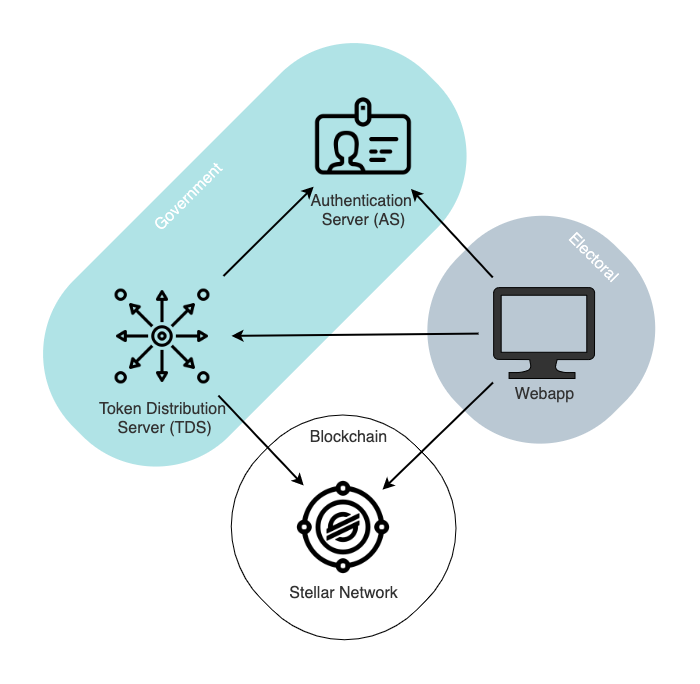
\includegraphics[width=9cm]{stellot-architecture.png}
\centering
\caption{Architecture of our e-Voting system}
\label{fig:architecture}
\end{figure} 
\iffalse

\begin{figure}
\begin{verbatim}
                          +                    +
         Government       |      Electoral     |      Blockchain
                          |                    |
                          |                    |
+-----------------------+ |                    |
| Authentication Server | |                    |
|         (AS)          | |                    |
+---------------------^-+ |                    |
                      |   |  +---------------+ | +-------------+   +---------+
                      +------> Client Webapp +---> Stellar     +---> Stellar |
                      |   |  +---------------+ | | Horizon API |   | Network |
   +------------------v-+ |                    | +-------------+   +---------+
   | Token Distribution | |                    |
   |     Server (TDS)   | |                    |
   +--------------------+ |                    |
                          |                    |
                          |                    |
                          +                    +
\end{verbatim}
\caption{Architecture of our e-Voting system}
\label{fig:ascii-box}
\end{figure} 
\fi

The big pictue of our system has been shown in Figure \ref{fig:ascii-box}.
The proposed system consists of three parties: Government, Electoral, and Blockchain. Both Government and Electoral distrust each other, because each of the parties has an interest in manipulating the process of election. Electoral demand from Government to be as transparent as possible. Government perform authentication and authorization process to prevent unauthorized votes or double \textit{vote token} issuance.

Ideally, Authentication Server (AS) and Token Distribution Server (TDS) should be separate entities, but we assume the pessimistic scenario, where they both cooperate to manipulate election results. Moreover, the system should consist only of a client webpage that allows users to interact with the Stellar network, getting rid of the centralized AS and TDS. Unfortunately, the proposed system requires a central authority for voter authentication, thus becoming a single point of failure. This flaw has been addressed at the end of this paper. There are also many proposals on how to achieve authentication on the blockchain ecosystem, but we won't cover them in this paper.

%JS tu bi sie przydało dokladniej opisac przeplyw danych miedzy wezlami ssytemu a nie tlko same role

%\subsection{Scalability}

Blockchain is famous for being very slow. Ethereum creator Vitalik Buterin claims that Blockchains face trillema ~\cite{ethereum} which allows them to choose only two of three properties: Decentralization, Security, and Scalability. 
And here is the place where a variety of different Blockchain platforms comes out offering something unique. While most conservative Blockchain like Bitcoin and Ethereum put on Security and Decentralization, others offer higher Scalability on the cost of Decentralization and Security. Stellar uses its own consensus protocol called Federated Byzantine Agreement(FBA) ~\cite{mazieres2015stellar}, which is decentralized variant of Byzantine Agreement consensus protocol, which is fast, cheap, has flexible trust model, doesn't require mining and is secure against adversaries with vast computational power (51\% attack).

%JS to troche niebezpiecznie pisac ze zaimplementowany system
%poswieca bezpieczenstwo kosztem skalowalnosc 
%trzeba by tu uzasadnic ze nie bedzie to mialo 
%wplywu na zaufanie do wynikow glosowania

As for the March 2020, Ethereum can process 15 transactions per second (TPS). Whereas Stellar can process 10 TPS, while each transaction can contain up to 100 operations.
%JS skad ta informacja \cite lub footnote
%JS co z tego wynika, jakie zalozenia co do wydajnosci systemow glosowania,
%jesli by przyjac ze wszyscy polacy moga glosowac
%i glosowanc beda po kolei w czasie (z rozkladem rownomiernym (co jest oczywiscie nieprawdziwe bo np rano mniej ludzi glosuje)
% to eterum przy 40 mln napewno sie przytka 10h* 3600 * 15

%\section{Authentication and Authorization}
Authentication and Authorization is provided by AS.
Voter obtains authentication token from AS using one of the available methods like OAuth2/OpenID Connect or Profil Zaufany 
as we do it in our approach. 
This token is then presented to TDS, who can authenticate the request by asking AS. Next, TDS checks in its local database, if such user has not already issued a vote token. Preventing from double \textit{vote token} issuance.

%\section{Vote Token}
We assume that the number of eligible voters is public information. Hence becoming the value of a maximum number of tokens in this election. After asset creation, issuing accounts have to lockout from creating a new asset, so all participants can be sure that no more tokens are ever created. Additionally, it should be impossible to perform vote, after the end of the election. Unfortunately Stellar doesn’t have such feature build-in, although it can be done by blocking all new token transfers from TDS to ballot-box account.
Assets in stellar blockchain, are divisible to 7 decimal points. This is an unwanted feature since we don’t want to allow users to vote by just one-tenth of their vote. To prevent it, we will treat 1 vote token as the smallest indivisible amount possible in XDR which is 1 scaled down by a factor of 10,000,000 (this format allows to represent decimal numbers in 7 digit precision, without introduction floating-point arithmetics and it’s innate errors).
Vote option is expressed in strictly encoded 32 byte MEMO field available in blockchain transaction. Frame structure is presented in Figure \ref{fig:ballot-encoding}. 
%JS co na rysunku jest? opisac



\begin{figure}
\begin{verbatim}
+----+-------------------------+-------------------------+---------------+
|Name|     #1 Answer code      |      #2 Answer code     | Random string |
+------------------------------------------------------------------------+
|    |                         |                         |               |
|Bits| A1=ceil(lg(|Answers1|)) | A2=ceil(lg(|Answers2|)) |  r=256-sum(A) |
|    |                         |                         |               |
+----+-------------------------+-------------------------+---------------+

\end{verbatim}
\caption{Voting ballot encoded in 32 byte MEMO field}
\label{fig:ballot-encoding}
\end{figure} 

We propose questions and options for multi-option ballots and further extensions.
The MEMO field is encrypted using the publicly available special public key,
preventing from preliminary results. %JS ????? nie jasne 

At the end of the election, the authorities publish corresponding private key, allowing everyone to calculate the election results on their own. A random string of bits is added to prevent preliminary results that could be achieved by summing equal memo fields.

\section{Privacy}
\label{privacy}
eVoting Privacy in  systems employing BlockChain 
technologies is the hardest problem to achieve. 
%JS dlaczego? cite nikt tego nie zrobił? jak inni to rozwiazywali odniesienie do state of the art
Especially in conjunction with authorization and data stored public blockchain. Additional procedures should be implemented to  solve this problem. 

The first one is to allow each voter to privately pick one authorization code which can then be attached to the transaction making it valid. Method which allows to achieve exactly this is called ANDOS (All-or-nothing-disclosure-of-secrets) ~\cite{andos} ~\cite{salomaa1990secret} ~\cite{applied_cryptography}. Unfortunately, it has some unacceptable flaw i.e. each voter has to communicate with all other voters. It is 
highly unpractical in public elections, but might be acceptable in smaller contexts. 
%JS czemu?

Another option to achieve voting   privacy is \textbf{blind signatures} ~\cite{applied_cryptography}. This technique makes it possible to sign encrypted (blinded) transaction and use the signature with the decrypted (unblinded) transaction. In other words, Alice can prepare her vote transaction, encrypt it, send it to Bob, who then sign it and send it back to Alice. As a result, Alice gets a valid signature without revealing her vote option. When Alice publishes such a transaction, Bob can not connect the previously signed transaction with Alice. 
There is one problem, Alice can prepare malicious transaction, send it to Bob, who then blindly sign the transaction. What is even worst, is the fact that Bob can not punish Alice, since he has already broken the link between her identity and such malicious transaction during blind signature.

\subsection{Cut-and-Choose protocol.}
\label{cut-and-choose}

Solution to  problem of preparing 
malicious transactions can be solved in the folowing way.  
Alice creates \(n\) (e.g. 100) random vote batch transactions. Batch consist of all possible vote options. If there is 6 candidates, and n equals 100, then we need to create 100 batches of 6 transactions each (600 transactions). Each batch gets blinded with different blinding factor. Alice sends them to Bob. Who challenges Alice for \(n-1\) unblinded batch of transaction. He uses them to validate their structure, especially if they don't try to issue more than 1 \textit{vote token} or perform any illegal operation. Then:

\begin{itemize}
 \item If any transaction is malicious, Alice loses her right to vote and optionally gets punished.

 \item If all of them are correct, he compute sign on the missing batch of transactions, and sends them back to Alice. She picks the sign that correspond to transaction of her choice, unblind it and add it to the transaction.
\end{itemize}

Bob does not know which transaction gets published to the network, because he's sign, will be transformed (unblinded) before adding to transaction while still keeping it's cryptography validity. In result, Bob can not connect Alice with her vote decision. In fact, he doesn't know anything about such transaction, but since he checked and validated randomly selected \(\frac{n-1}{n}*100\%\) previous transactions, he can assume with high probability that this one is also not malicious.

There are two problems with this method.
First, there are \(\frac{1}{n}*100\%\) chance that Alice will succeed in cheating. In the case where she steals all vote tokens, the election must be remade, because no more tokens can be issued from the distribution account. Additionally, no consequences can be made to such an attacker, because we have broken the link between the user and the transaction during blind signature. Introducing punishment for attacker who try to perform malicious transaction seems to be negligible, because when Alice gets challenged to unblind malicious transaction, she may just not respond, preventing from revealing the content of such transaction. In such a case Bob should block on the challenge, preventing Alice from "taking another try in the lottery".
In such a way  we get protocol that achieves voter anonymity requirement.

%Here is the  blind signature implementation for ECDSA [https://github.com/oleganza/bitcoin-papers/blob/master/BitcoinBlindSignatures.md]
%Another post on Schnorr/DSA https://blog.cryptographyengineering.com/a-note-on-blind-signature-schemes/
% My question: https://crypto.stackexchange.com/questions/77558/ed25519-blind-signature
% sodium implementation https://github.com/dchest/tweetnacl-js/blob/5bf1ff5fa15e89ae249401b0d5aa54c5c5955041/nacl.js#L1076



\section{Blind signature implementation}

To achieve vote anonymity, we use the rules described in section ~\ref{privacy} \nameref{privacy}. Voter start interactive session with Issuer where they proceed Chaum blind signature \cite{blindsignatureschaum} on ed25519 scheme. 

Let's assume Alice to be Voter, Bob to be Issuer, P to be Bob public key, H to be hash function, || to be concatenation operator, M to be the \textit{vote token transaction} from TDS to the ballot-box.
This process consists of following steps:
\begin{itemize}
\item Bob generate random nonce number \textit{k} in the range $(1, q-1)$, compute 
\(r = G^k \pmod{p}\)
and sends it back to Alice.
\item Alice picks two random numbers \textit{a} and \textit{b} in the range (1, q-1), use them to compute challenge number \textit{e}
\[R' = r*(G^a)*(P^b) \pmod{p}\]
\[e' = H(R’|| P || M)\]
\[e = e' + b \pmod{q}\]
and send it back to Bob
\item Bob signs it 
\(s = e*x + k \pmod{q}\)
and send it back to Alice
\item Alice computes 
$s' = s + a \pmod{q}$
The pair (R', s') is a valid signature on transaction M.
\end{itemize}
Alice gets valid signature on transaction M, while Bob knows only \textbf{blinded hash} of the transaction M.
This process can be visualized as:
\begin{itemize}
    \item Alice prepares a voting ballot.
    \item Place it into the envelope along with carbon paper.
    \item Ask Bob to sign the envelope.
    \item Alice removes envelope and carbon paper.
    \item Alice cast the ballot into the ballot box.
\end{itemize}

To protect the Bob from signing a malicious transaction, we use the cut-and-choose technique described in section \ref{cut-and-choose}.

Since the signature on the transaction (ballot) is valid, Alice can publish it directly to the stellar network, and track it with the received transaction id. 

%\section{Scalability Issue - Sequence Number - Draft}
%Each Stellar account has it's own transaction counter called sequence number. Once the transaction is submitted to network, the next transaction has to be submitted with incremented sequence number, otherwise it will be rejected. This is very troublesome in our use case, because, when the TDS sign two transactions for two users, the second one, can not publish it's transaction, before the first doesn't do so. It could be mitigated by introducing some kind of time frames for each user, but it would significantly limit the number of transactions per second and would allow TDS to identify transaction submission with time frame, compromising privacy.
%Instead we use concept called Channels. Channel is simply a intermediary account that provides his sequence number to process transaction on someone else behalf. Those channel accounts could be managed by TDS and allocated for each new transaction request. Unfortunately, when we get privacy of such process into account, it turns out that TDS could easly associate channel with our identity, striping us from previously acquired anonymity. 
%We could allow user to create new channel account, for each batch of transactions during blind-signature process. Here we face with another problem, which is the fact, that the channel account is responsible to pay the transaciton fee. Thus, such account has to be funded prior to providing intermediary service. Funding has to be done with the same care as vote transaction, since they are equally capable of breaking privacy. 
%% lack better word for "capable of breaking privacy", any suggestions ?

%\paragraph{TDS publish channel funding}
%Additionally the funding transaction has to be published to the network by TDS. Otherwise we are back to be origin problem of sequence number blocking. But if the transaction is published by TDS, it is able to identify us by the channel used to pass the transaction trought. He allocate us the channel, so he knows exactly who will pass the transaction through it, so the blind signature losses it's privacy value.

%\paragraph{User publish channel funding}
%User generate new x random channel account keypairs, for each of them, create transaction funding this channel, sends them to TDS, who allocate for him channel from channel pool to perform blind-transaction on my-channel funding transaction. Then, we don't instantly redeem this transaction to fund my channel, because in the next step (vote transaction) the TDS could determine what transaction uses already created channel and which don't. So I send him random-channel-throught-vote-transaction to perform blind signature. And now I can publish create-channel-transaction, followed by vote transaction. 
%Problem: if the TDS assign unique funding-channel for each voter, then he can identify voter with his vote by associating the transaction that was send throughout that channel. So we lose privacy !

%\paragraph{3rd party publish channel funding}
%3rd party that voting host has no connection to, publish channel funding. 


\section{Transaction Fees}
We evaluate the proposed system in the context of transaction fees. To do this we can estimate how much would cost the 2019 Polish parliamentary election, handled by the proposed system. We already know that 18 470 710 people participated in such an election. Each operation on the stellar network costs 0.00001XLM. Our vote transaction consists of just one operation (transfer of 1 \textit{vote token}, and so the total cost of the transaction also equals 0.00001XLM. We know that the closing price for one Lumen in the day of the election was 0.061 USD. We can easily calculate \(18470710 vote * 0.00001 \frac{XLM}{vote} * 0.061 \frac{USD}{XLM} \approx \textbf{11,27 USD}\). Other operational transactions can be neglected due to the very low influence on the total sum.

\section{Securing webapp}
Hijacked become single


\section{Preparation}
To create such an election, we need an distribution account, ballot-box account, and a new vote token. Variables that need to be propagated in backend and webapp code are:
• asset name, asset issuer keypair, distribution keypair and ballot-box keypair. (webapp receives only public part of keypairs)
• limit of possible vote tokens (number of eligible voters). 
• list of (candidate name, candidate code).
• keypair for encrypting/decrypting transaction MEMO fields before/after election end.
%JS rysunek + ospis


\section{Fully Decentralized Blockchain Application}
In the blockchain world to ensure absolute trust, everything should be blockchain contained, which is often hard, impractical and/or expensive. For example, one could encode all eligible voter addresses or some special one-time codes, in the smart contract, and then allow redeeming vote token only to addresses/codes which are present in there, very similar to traditional election system where all eligible voters are listed on paper. The ballot is issued only if the elector is present on such list. While this might work for a small list of addresses, it can become overkill for election when the cost of such a huge smart contract is taken into account. Fortunately, there are already blockchains that allow linking data from outside the blockchain, by using Oracles. To ensure immutability and integrity, such list can be hosted on IPFS (Content Addressed Network) where data is identified by its hash. Unfortunately, Stellar doesn't have such a feature yet. Right now, only part of the system is decentralized. Since this system relies on a centralized AS, it inherits it's property too. Fig. 3 present the centralization/decentralization parts of the system.

\begin{figure}
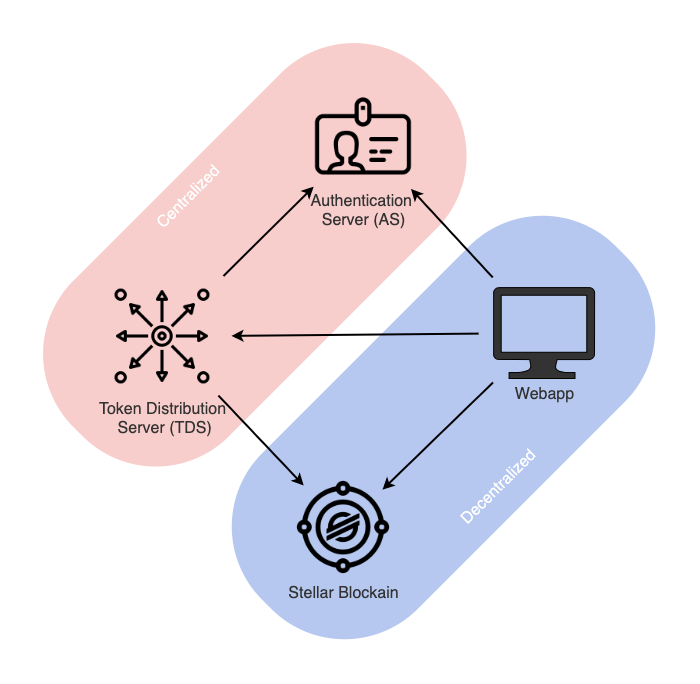
\includegraphics[width=9cm]{stellot-decentralization.png}
\centering
\caption{Centralized and decentralized parts of the system}
\label{fig:decentralization}
\end{figure} 


%\section{System weakness}

\section{Discussion and Future Works}


%podsumowac co sie udało zrobic, jakie są główne osiągnięcia przedstawione w artykule
%JS Future works :wdrozenie na eti
The proposed system satisfies all outlined requirements. Each vote is recorded on Blockchain, and everyone can calculate election results without trusting authorities. Thanks to a blind signature, Voter can be sure that his decision will be kept private. Unfortunately, the system still relies on trust to the issuer, who decide who is eligible to receive vote right. If this single point of failure could be eliminated, we would achieve a truly decentralized trustless system, without central authorities.


It should be noted that, we assumed that AS and TDS are honest actors,
and we know the total number of eligible voters and that only eligible voters can redeem tokens. The question is how can we know if the authorities don't publish a greater number of eligible voters and redeem this extra number of tokens to themselves. Being able to significantly influence the election results. The pre-registration phase doesn't help here, since the malicious government also can take part in it, generating extra tokens. There is some mitigation proposition where it would be required from voters to compute some kind of proof-of-work that would require a lot of computing power by one actor to create a lot of votes.

With our system we show how blockchain can be used not only for cryptocurrencies, but also in assets tokenization and as a part of trusted system where it acts as immutable, verifiable and transparent database. Stellar is just one of many platforms that could be used in such cases, but it turns out that it handles it very well. What makes Stellar one of the best
options in this category is speed and transaction fees. We estimated the costs of the 2020 Polish parliamentary election to 11,27 USD. 
To estimate transaction speed we would need to host a local instance of Stellar Horizon API server to isolate from network latency and possible queuing overhead. Doing it would also allow us to accurately measure how the proposed system behaves on heavy overload. 
It would be interesting to compare such systems on different blockchain platforms. 
We provide general-purpose voting platform demo at \url{https://voting.stasbar.com} with its source code at \url{https://github.com/stasbar/stellar-voting}.
Starting with the general-purpose voting platform, we would like to target all kinds of votings including domain-specific elections, straw polls, referendums, plebiscites. We believe that our goal is also to digitize the academic/government votings. Such elections require domain-specific applications, and so we would like to create a framework for these types of solutions. Especially the Auth-Server is something that will differ in every institution. We plan to test such system first at our University. When applied successfully, we will scale the product to other domains. 


\bibliographystyle{splncs04}
\bibliography{refs}
\end{document}
